
%%******************************************************************************
%% SECTION - Materials 
%List everything needed to complete your experiment.
%%******************************************************************************



\subsection{Materiais}
Os materiais utilizados para a execução do experimento do sensor indutivo na
Usina foram:
\begin{itemize}
  \item Três sensores indutivos;
  \item Cabos M12 com conectores submarinos e umbilical com saída de backup;
  \item Eletrônica embarcada à prova d'água composta por: tubo metálico, duas
  baterias, chave de ativação, placa eletrônica customizada e cabeamento;
  \item Ferramentas da eletrônica: voltímetro e modem;
  \item Computador com sistema operacional Ubuntu e Modem Ethernet;
  \item Estrutura mecânica para acoplamento do sensor; 
  \item Ferramentas: chave de fenda e de boca 8mm;
\end{itemize}
Os sensores indutivos NBB20-L2-E2-V1 adquiridos na Pepperl-Fuchs foram
previamente testados em laboratório nas condições que se esperava encontrar em
JIRAU (ver relatório Testes de Laboratório, seção do sensor indutivo): objetos
metálicos em torno do sensor, sensor dentro e fora da água, distância de 20 a 30mm do objeto a ser detectado.

Os cabos M12 de 4 vias e 5m de comprimento, também adquiridos na Pepperl-Fuchs,
foram estendidos com cabos que se conectam ao tubo da eletrô\-nica embarcada.
As extensões são do tipo submarina, capaz de resistir a altas pressões embaixo
d'água. 

O cabo umbilical da eletrônica embarcada apresenta 12 vias, onde duas são as
saídas de sinais dos sensores indutivos. Essas saídas garantem a
verificação dos sensores indutivos caso haja falha do dispositivo GPIO/Ethernet
da placa eletrônica. A ferramenta utilizada para essa verificação é o
voltímetro.

A eletrônica embarcada do teste em JIRAU é um protótipo simplificado da
eletrônica final do projeto ROSA. Ela pode ser subdividida em projeto
mecânico, placa eletrônica e potência. 

A estrutura mecânica da eletrônica embarcada deve atender aos seguintes
requisitos de projeto: imersível 100m em água, resistente à vibração, resistente a choque
mecânico e acoplamento simples à viga pescadora, isto é, sem causar alterações à
estrutura. A solução rápida e simples adotada foi a montagem e adaptação do
antigo tubo do projeto LUMA, ROV com expedição Antártida~\ref{fig:tubo}. 

\begin{figure}[H]
 \centering
 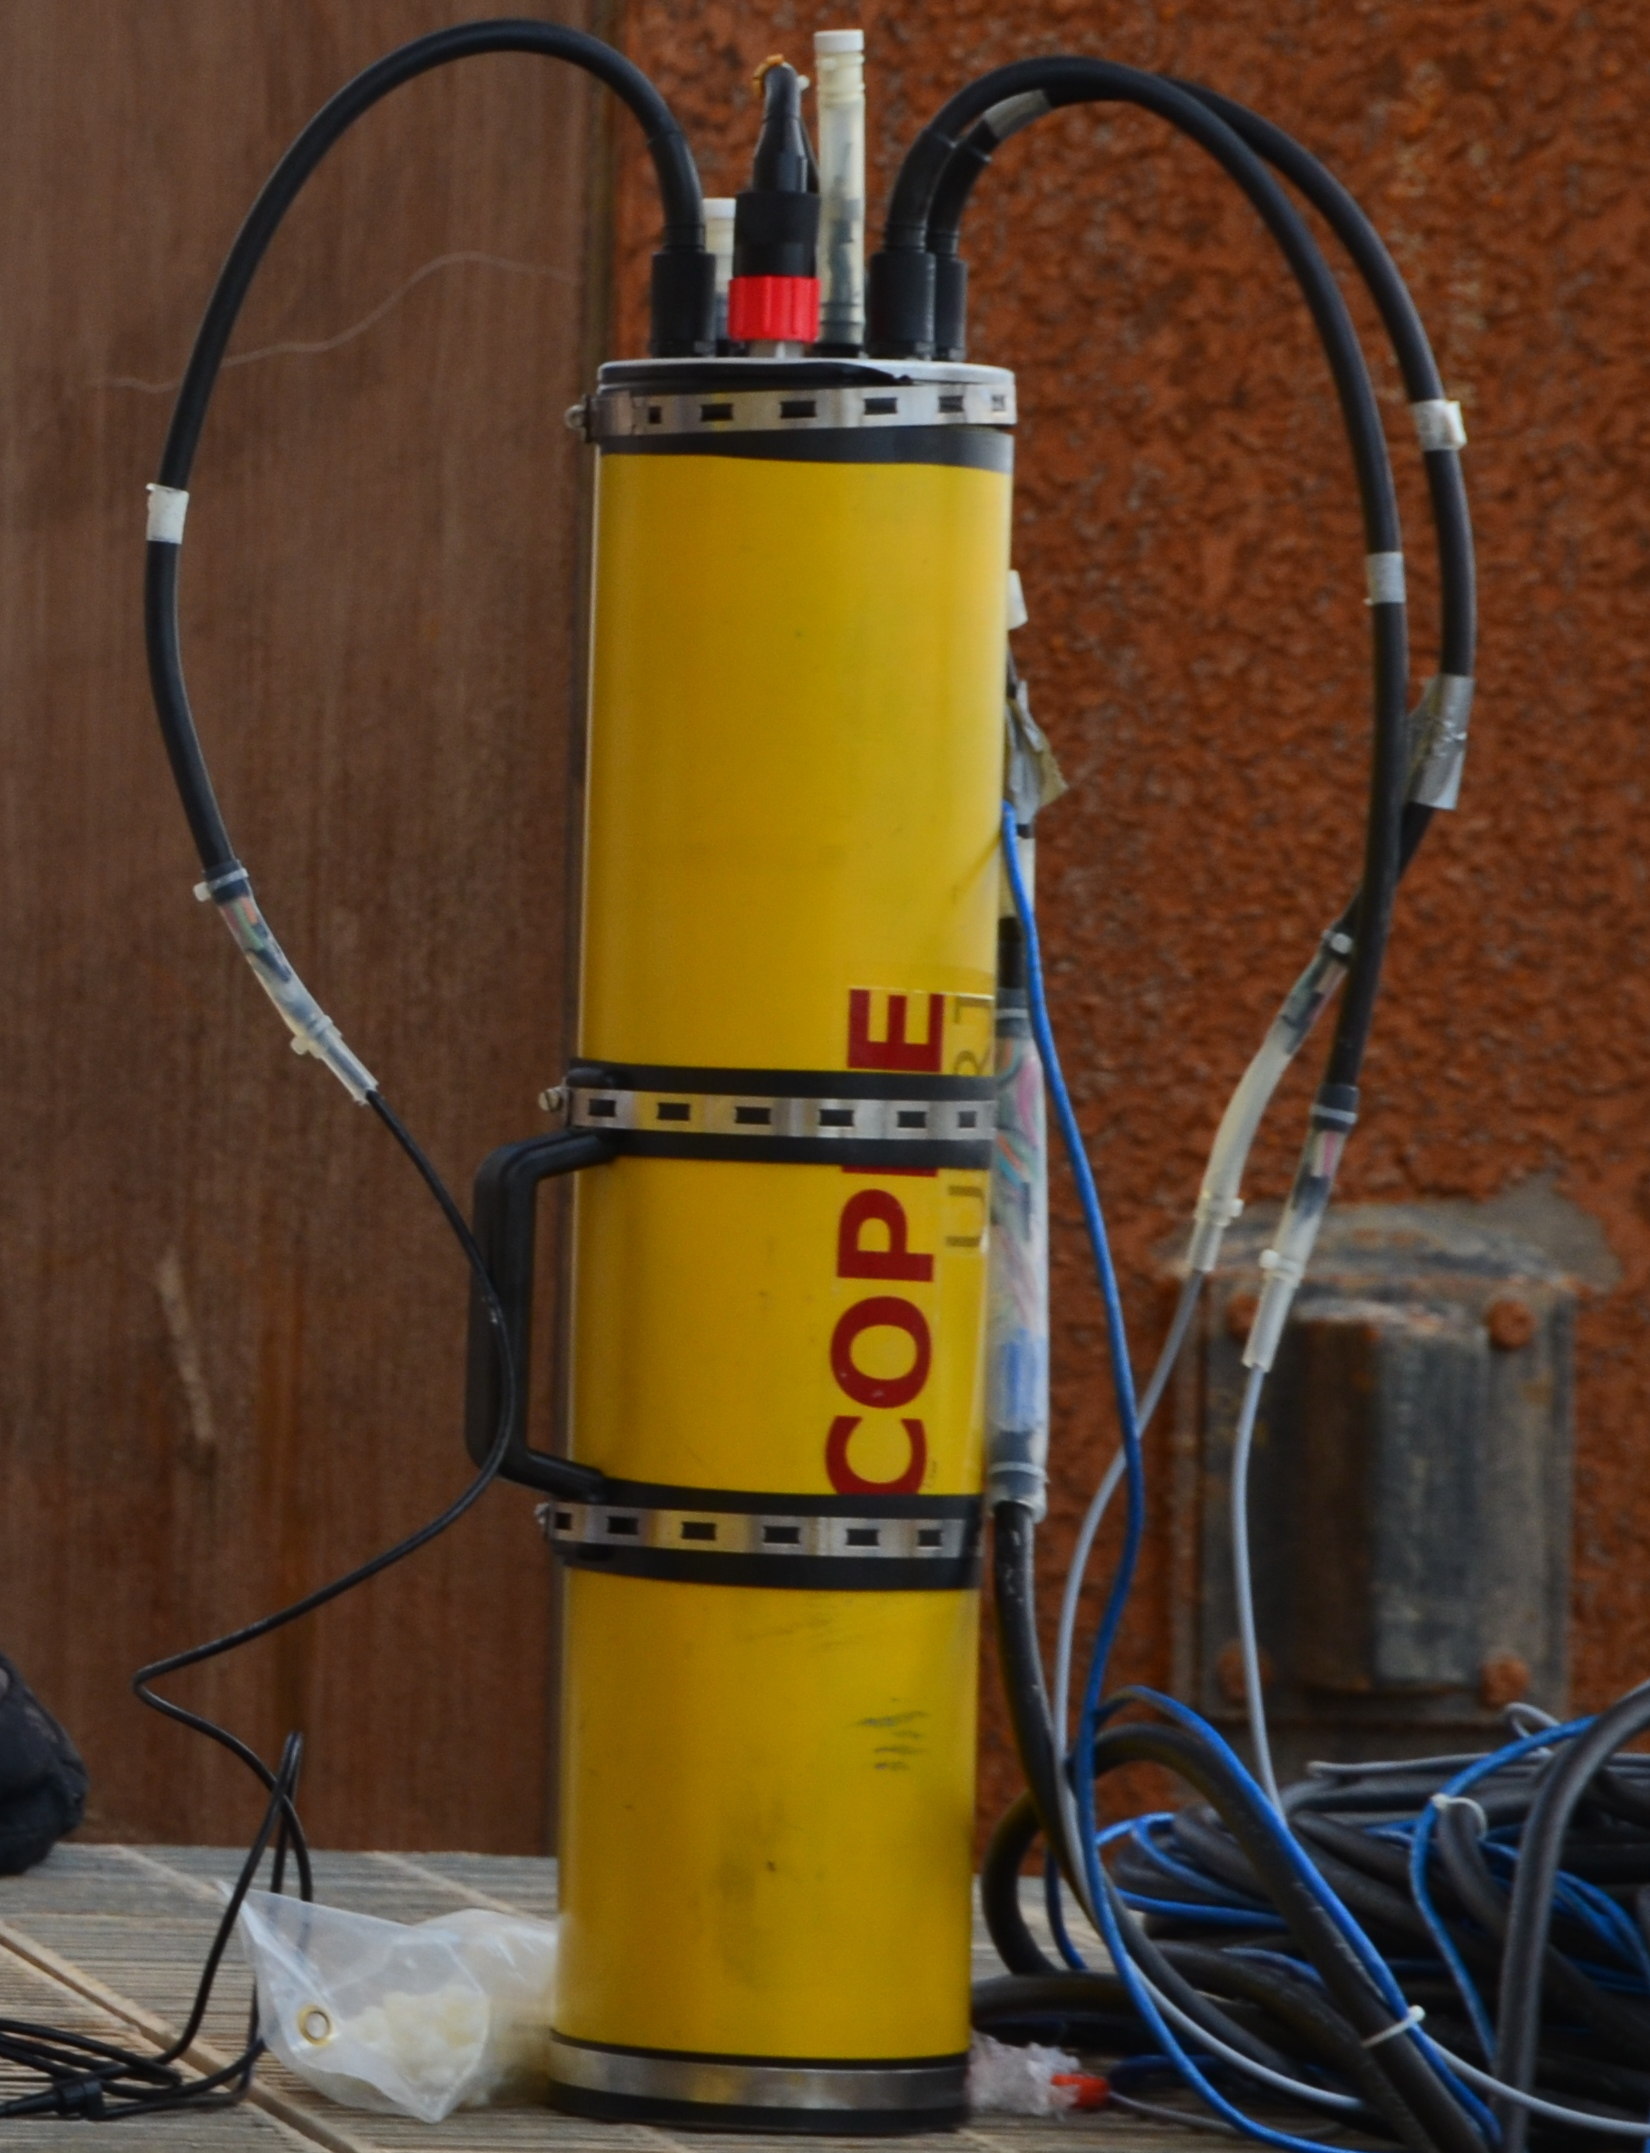
\includegraphics[width=1\columnwidth]{indutivo/figs/tubo.jpg}
 \caption{Tubo da eletrônica embarcada}
 \label{fig:tubo}
 \end{figure}

A placa eletrônica customizada é responsável pela distribuição e conversão da
potência, comunicação e conversão do meio físico entre dispositivos através de
um dispositivo GPIO/Ethernet. A entrada para sensor indutivo na placa eletrônica
é um conector de 4 vias, onde apenas 3 são utilizadas: potência $24V$
diretamente da bateria ou fonte externa, aterramento (Ground da bateria ou fonte
externa) e sinal. O sinal é uma saída do tipo relé, ou seja, $24V$ quando há
proximidade faceada com metal. A saída, então $24V$, passa por um conversor de
tensão, o que garante uma queda para $3.3V$. Um dispositivo GPIO/Ethernet
converte a saída de nível lógico TTL para Ethernet. Vale ressaltar que a
conexão da placa ocorre com os conectores internos do tubo, estrutura mecânica,
e não diretamente com o cabo do sensor indutivo. A lógica da montagem é: sensor
indutivo - Cabo M12 - Emenda cabo externo do tubo - Conector tubo - Cabo interno do tubo - Conector placa - Placa.

O computador com sistema operacional Ubuntu recebe os dados via Ethernet pelo
Modem. O sistema para obtenção dos dados foi desenvolvido em ROCK.

A potência da eletrônica embarcada é fornecida por duas baterias $12V$, $7AH$ em
série, o que garante um total de $24V$. Elas são alojadas internamente ao tubo,
podendo ser desligadas por uma chave externa ao tubo, com proteção à prova
d'água FIGURA. O projeto ainda possibilita a entrada de uma fonte externa de
alimentação por uma das saídas do umbilical, em caso de falha nas baterias.

A estrutura mecânica para acoplamento do sensor foi desenvolvida pelo prof.
Ramon e pode ser observada na FIGURA. O formato da barra acompanha a lateral
da garra pescadora, oposta à pegada com o stoplog. Na barra ortogonal à
primeira, localizada na parte inferior, é acoplado o sensor indutivo, garantindo
sua proteção em relação ao olhal do stoplog. O acoplamento à viga pescadora foi
realizado com abraçadeiras durante a montagem.




\label{materials}




